\section{YogaAlign Dataset}
\label{sec:dataset}

We construct \textbf{YogaAlign}, a geometry-grounded vision--language benchmark that extends Yoga-82 with reconstructed 3D body structure, geometric measurements, and instruction-style question--answer (QA) annotations.
The benchmark supports reasoning beyond pose recognition, including joint-angle interpretation, bilateral comparison, regional alignment analysis, and pose-specific instructional knowledge.
At a high level, we construct it in three stages as follows.
We reconstruct a 3D body from each image, then extract geometric descriptors, and finally generate two QA sets grounded in either pose-level textual knowledge or image-specific geometry.

\subsection{Source Images and 3D Body Reconstruction}
\label{subsec:source_reconstruction}

\noindent\textbf{Yoga-82 source dataset.}
YogaAlign is built on Yoga-82~\cite{verma2020yoga82}, which contains 28,478 images spanning 82 fine-grained yoga-pose categories.
The images were collected from online sources and exhibit substantial variation in viewpoint, background, illumination, clothing, practitioner appearance, and execution style.
Yoga-82 is therefore a challenging setting for geometry-aware reasoning.
Many poses differ through small changes in limb articulation, trunk orientation, balance, or bilateral symmetry.
The original dataset, however, provides only RGB images and category labels.
It does not include 3D body structure, geometric measurements, or language annotations.

\noindent\textbf{Monocular body reconstruction.}
We recover a 3D body representation from each Yoga-82 image using the pretrained SAM 3D Body model~\cite{yang2026sam3dbody}.
Given an image $I$, the model predicts an articulated body and surface mesh under the Momentum Human Rig (MHR) representation.
We retain the predicted mesh vertices and anatomical keypoints required by the subsequent measurement stage.
Fig.~\ref{fig:sam3d_examples} shows the reconstruction of one image from each category.

\begin{figure*}[!t]
    \centering
    \includegraphics[width=0.98\textwidth]{_ALL_CLASSES_GRID.png}
    \caption{SAM 3D Body reconstruction of one image from each of the 82
    Yoga-82 categories. The recovered bodies span standing, seated, supine,
    inverted, twisting, and arm-balancing configurations. We extract geometric
    descriptors across this full range.}
    \label{fig:sam3d_examples}
\end{figure*}


We treat the recovered bodies as reconstruction-derived geometric proxies.
The reconstructions are not motion capture or manually verified biomechanical ground truth.
Their accuracy may be affected by self-occlusion, foreshortening, loose clothing, unusual inversions, left--right ambiguity, and monocular depth uncertainty.

\subsection{Geometric Measurement Extraction}
\label{subsec:geometric_measurements}

Dense meshes are expressive but too high-dimensional for language-grounded pose analysis.
We therefore reduce each reconstruction to a compact set of anatomically interpretable descriptors (Table~\ref{tab:geometric_metrics}).
We map the raw coordinates to a canonical frame before measurement.
Centering the vertices and keypoints at the mesh centroid removes global translation, and a fixed 3D coordinate convention supplies a consistent vertical axis.

\begin{table*}[t]
\centering
\caption{Taxonomy of geometric descriptors extracted from reconstructed 3D bodies.}
\label{tab:geometric_metrics}
\small
\setlength{\tabcolsep}{4pt}
\renewcommand{\arraystretch}{1.16}
\begin{tabularx}{\textwidth}{L{0.17\textwidth} L{0.25\textwidth} L{0.27\textwidth} X}
\toprule
\textbf{Group} & \textbf{Descriptors} & \textbf{3D computation} & \textbf{Reasoning target} \\
\midrule
Limb flexion &
Left/right knee and elbow flexion &
Interior angles of hip--knee--ankle and shoulder--elbow--wrist triplets &
Degree of flexion and left--right comparison. \\
Limb opening/elevation &
Left/right hip opening and shoulder elevation &
Angles between limb segments and torso-level reference axes &
Hip opening and arm elevation. \\
Trunk geometry &
Trunk tilt, lateral bend, twist, and neck alignment &
Pelvis--shoulder, shoulder--hip, and neck--torso directions &
Uprightness, lateral inclination, axial rotation, and head--torso consistency. \\
Bilateral symmetry &
Knee, elbow, and hip symmetry; shoulder and hip height offsets &
Left--right angular differences and normalized vertical offsets &
Symmetric or asymmetric execution across corresponding body regions. \\
Balance/support &
Stance width and body-center offset &
Ankle separation and horizontal displacement of the mesh center from the pelvis midpoint &
Base of support and lateral body shift. \\
\bottomrule
\end{tabularx}
\end{table*}

\noindent\textbf{Joint-angle descriptors.}
For three anatomical keypoints $\mathbf{p}_a$, $\mathbf{p}_b$, and $\mathbf{p}_c$, we compute the angle centered at $\mathbf{p}_b$ as
\begin{equation}
\theta(a,b,c)=
\cos^{-1}\!\left(
\frac{(\mathbf{p}_a-\mathbf{p}_b)^{\top}(\mathbf{p}_c-\mathbf{p}_b)}
{\lVert\mathbf{p}_a-\mathbf{p}_b\rVert_2
 \lVert\mathbf{p}_c-\mathbf{p}_b\rVert_2}
\right).
\label{eq:joint_angle}
\end{equation}
Knee flexion is measured from the hip--knee--ankle triplet, whereas elbow flexion is measured from the shoulder--elbow--wrist triplet.
Hip opening and shoulder elevation are computed relative to torso-level reference axes.
\begin{figure*}[t]
    \centering
    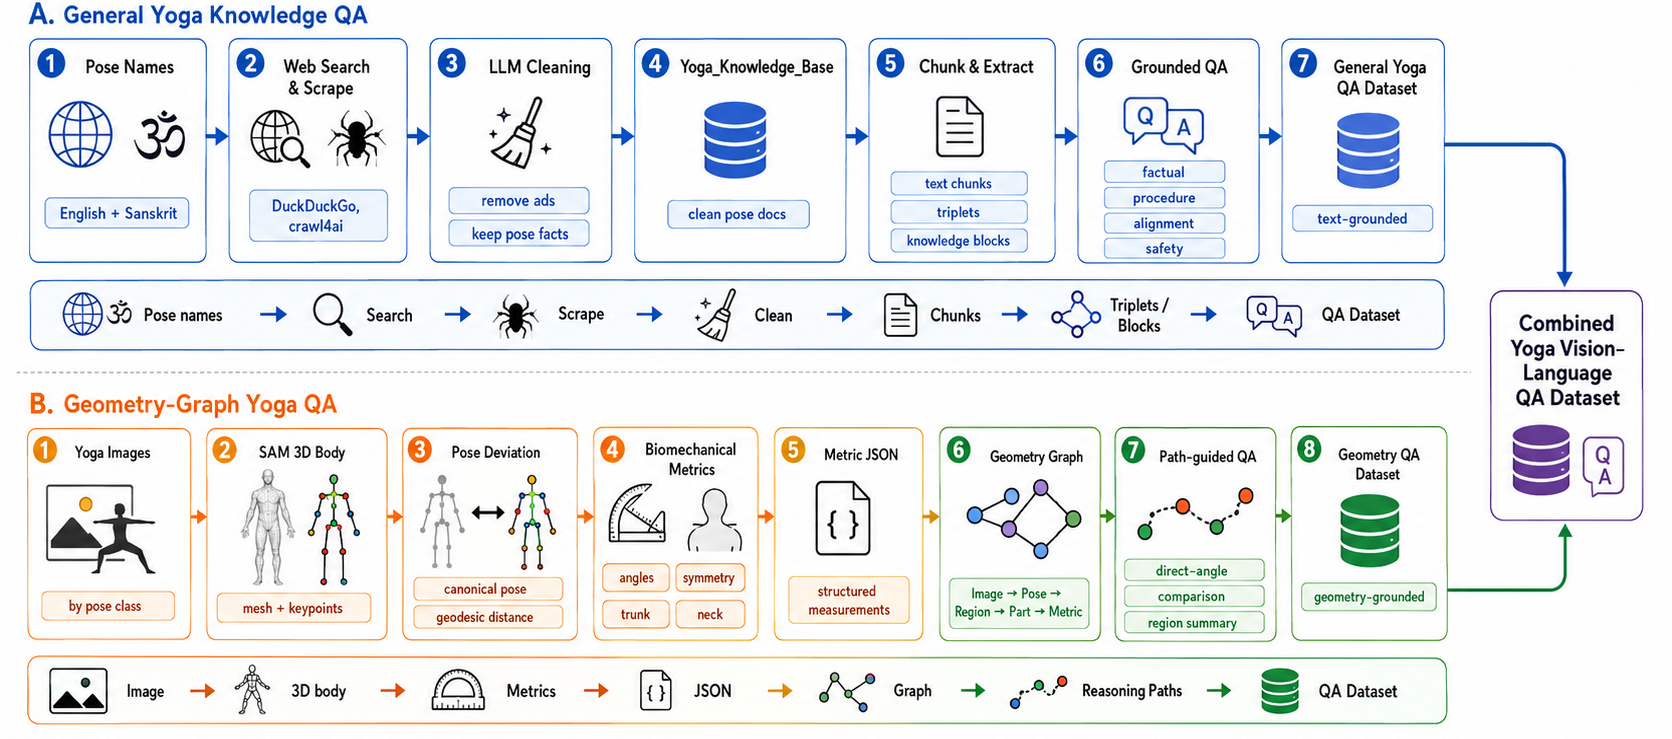
\includegraphics[width=\textwidth]{fig_dataset.png}
    \caption{\textbf{YogaAlign dataset construction.}
    Pose-level domain knowledge and image-specific 3D geometry are processed
    separately to produce the domain-knowledge and geometry-grounded QA
    annotations.}
    \label{fig:dataset_construction}
\end{figure*}
\noindent\textbf{Trunk, symmetry, and support descriptors.}
Trunk measurements are derived from the pelvis--shoulder axis and the shoulder--hip and neck--head directions.
Bilateral descriptors quantify differences between corresponding left and right measurements.
Scale-dependent quantities (stance width, shoulder-height offset, and hip-height offset) are normalized by the vertical extent of the reconstructed mesh to reduce sensitivity to body and reconstruction scale.

\noindent\textbf{Structured metric records.}
Each image is paired with a record containing the descriptor name, anatomical region, numeric value, unit, definition, and discretized interpretation state.
Fixed thresholds map continuous measurements to language-compatible states such as \emph{nearly straight}, \emph{deeply bent}, \emph{upright}, \emph{rotated}, or \emph{asymmetric}.
The states keep the wording consistent, and the underlying numeric values preserve exact supervision.
We use the measurements only as reconstruction-derived alignment indicators for dataset construction.
The measurements are not intended as clinical, diagnostic, or rehabilitation measurements.

\subsection{Question--Answer Annotation}
\label{subsec:qa_generation}

YogaAlign contains two complementary QA sets.
The \emph{domain-knowledge} set captures pose-level semantic and instructional information that cannot be inferred reliably from body geometry alone.
The \emph{geometry-grounded} set expresses image-specific angular evidence extracted from the reconstructed body.
Table~\ref{tab:qa_annotation_overview} in Appendix~\ref{app:annotation_sets} contrasts their evidence sources and supervision targets.


\subsubsection{Domain-Knowledge QA Generation}
\label{subsubsec:domain_qa_generation}

For each of the 82 categories, we collect pose-relevant text from online sources into one document per asana.
The collected text is noisy, and we do not generate QA pairs directly from it.
An LLM extractor $E_{\phi}$ first converts each document chunk $c_i$ into relational facts $R_i$ and structured knowledge units $B_i$, and an LLM generator $G_{\psi}$ conditions on both:
\begin{equation}
\mathcal{Q}^{\mathrm{dom}}_i=G_{\psi}\bigl(c_i,E_{\phi}(c_i,p),p\bigr),
\label{eq:domain_qa}
\end{equation}
where $p$ denotes the pose.
Each accepted item stores its supporting facts, knowledge units, and an evidence phrase, so every answer remains traceable to the source text.
We instruct the extractor to keep only statements supported by the current chunk and to drop claims that a pose cures or treats a medical condition.
Both restrictions are carried by the prompt alone.
No independent check enforces either one, and we have not audited the retained records for unsupported medical claims.
Appendix~\ref{app:domain_generation} describes the collection, chunking, and deduplication procedure, and Table~\ref{tab:domain_qa_config} lists the values used.
We fixed these values before generation and did not search over them.

\subsubsection{Geometry-Grounded QA Generation}
\label{subsubsec:geometry_qa_generation}

The second set is generated directly from the measurements associated with an individual image.
We restrict this set to degree-valued descriptors, which provide continuous targets.
Non-angular normalized quantities, including stance width, body-center offset, and shoulder- and hip-height differences, remain part of the geometric annotation taxonomy but are not used for geometry-QA generation or angle-regression supervision.

\noindent\textbf{Metric facts and geometry graphs.}
For image $I$, each valid measurement $m\in\mathcal{M}_I$ is converted to a single metric fact
\begin{equation}
f_m=(r_m,b_m,n_m,v_m,s_m),
\label{eq:metric_fact}
\end{equation}
where $r_m$, $b_m$, and $n_m$ identify the body region, body part, and descriptor.
The entries $v_m$ and $s_m$ store the angular value and its discretized interpretation state.
We organize these facts into a graph $\mathcal{G}_I=(\mathcal{V}_I,\mathcal{E}_I)$ containing image, pose, region, body-part, metric, and interpretation nodes.
Edges encode relations such as image--pose, region--body-part, body-part--metric, and metric--interpretation.
The graph makes the available evidence explicit and supports controlled sampling of different reasoning structures.

\noindent\textbf{Evidence-path construction.}
We derive five path families from each graph (Table~\ref{tab:geometry_path_types}).
A path specifies the selected measurements, the intended reasoning behavior, and the evidence that must appear in the answer.
Direct paths target one descriptor.
Comparison paths pair corresponding left and right descriptors.
Regional paths combine multiple measurements.
Misconception paths verify a proposed condition.
Instructor-observation paths express a notable measured property.

\begin{table*}[t]
\centering
\caption{Evidence-path families for geometry-grounded QA generation.}
\label{tab:geometry_path_types}
\small
\setlength{\tabcolsep}{4pt}
\renewcommand{\arraystretch}{1.14}
\begin{tabularx}{\textwidth}{L{0.20\textwidth} L{0.27\textwidth} L{0.28\textwidth} X}
\toprule
\textbf{Path type} & \textbf{Evidence} & \textbf{Reasoning behavior} & \textbf{Answer constraint} \\
\midrule
Direct angle & One angular metric and its state & Read and interpret a measured angle & Include the body part, exact value, and interpretation. \\
Comparison & A paired left--right metric & Compare corresponding body parts under a predefined rule & Include both values and the resulting comparison. \\
Region summary & Multiple metrics from one region & Integrate a lower-body, upper-body, or trunk--neck configuration & Combine all selected values coherently. \\
Misconception & Metrics relevant to a proposed condition & Confirm or reject an alignment statement & State the decision and cite the required values. \\
Instructor observation & A notable metric and severity state & Express a teacher-style observation & Describe the measured property and cite its value. \\
\bottomrule
\end{tabularx}
\end{table*}

For knee and elbow comparisons, the smaller interior angle denotes the more flexed side.
For hip opening and shoulder elevation, the larger value denotes the more open or elevated side.
These deterministic rules keep the stated comparison direction consistent with the recorded values.
They do not validate the values themselves and inherit any left--right ambiguity in the underlying reconstruction.

\noindent\textbf{Memory-aware sampling and synthesis.}
We select 3,000 images using balanced-proportional sampling and generate two QA records per image.
One record emphasizes direct numeric supervision.
The other is drawn from a higher-order path family.
A rolling memory tracks recent path types, path identifiers, metric sets, question families, and normalized question signatures.
We penalize candidate paths for recent or frequent reuse.
The penalty reduces template collapse and improves coverage across reasoning forms.

For a selected path $p_k$, the generator receives its evidence $E(p_k)$ and recent generation history $h_k$:
\begin{equation}
(q_k,a_k)=G_{\psi}\bigl(p_k,E(p_k),h_k\bigr).
\label{eq:geometry_qa}
\end{equation}
The prompt requires the pose name in the question and every selected angular value in the answer.
It prohibits internal identifiers and unsupported spatial or biomechanical claims.
The model therefore puts a predefined evidence path into words.
It does not infer unrestricted yoga knowledge.

\noindent\textbf{Validation and numeric targets.}
We check each candidate QA pair against rule-based criteria for pose-name presence, required numeric values, left--right consistency, prohibited internal terms, path-specific constraints, and near-duplicate questions.
Failed samples are regenerated at most twice, with the violated criteria supplied to the generator.
If both regenerations fail, we use a deterministic evidence-based template.
Each accepted record stores
\begin{equation}
\bigl(I,q_k,a_k,p_k,E(p_k),\mathcal{A}_k\bigr),
\label{eq:geometry_record}
\end{equation}
where $\mathcal{A}_k$ contains the metric identity, body part, body region, exact value, unit, interpretation, and summary for every supervised angle slot.
This representation supports both language instruction tuning and continuous angle-slot supervision while retaining a traceable link to the underlying reconstruction-derived evidence.
Table~\ref{tab:geometry_qa_settings} in Appendix~\ref{app:generation_settings} lists the sampling and decoding values for this set, again fixed in advance.

\subsection{Dataset Composition}
\label{subsec:dataset_composition}

The final YogaAlign corpus contains 4,090 pose-level domain-knowledge examples and 6,000 image-specific geometry-grounded examples, 10,090 QA records in total.
The geometry set comprises 3,000 direct-angle, 905 comparison, 900 regional-summary, 600 misconception, and 595 instructor-observation records.
The two sets provide distinct supervision.
The domain set captures what is generally known about an asana, whereas the geometry set describes the measured configuration of a particular reconstructed body.
This distinction is retained throughout training and evaluation so that pose-level knowledge is not conflated with image-specific geometric evidence.
